\documentclass[UTF8,a4paper,10pt,twocolumn]{ctexart}
\usepackage[margin=1.7cm]{geometry}
\usepackage{amsmath,amssymb,booktabs,graphicx,xcolor,url}
\usepackage{tikz,pgfplots}
\usetikzlibrary{positioning,fit,arrows.meta}
\pgfplotsset{compat=1.18}
\setlength{\columnsep}{0.65cm}
\newcommand{\method}{LockPusher}
\title{LockPusher：基于状态隔离世界模型的对象适配，用于关节锁定下的推动}
\author{匿名作者}
\date{}
\begin{document}\maketitle

\begin{abstract}
在递归推动模型中，对象状态的修正可能通过反馈改变后续机器人预测。我们研究已诊断关节锁定下的这一适配问题：在保留指定机器人预测器的同时，更新物体响应。LockPusher将解析锁定投影与独立的参考、干预滚动相结合。两条分支分别维护自身状态与记忆，返回的机器人坐标来自参考分支，物体坐标来自干预分支。在分支确定、初始条件及候选动作匹配时，整个滚动过程中的机器人与推杆预测均与投影后的参考一致。覆盖三个历史检查点、三种动力学条件和三个预测时域的27组配对比较表明，选择性输出保留了干预模型相对参考模型平均16.74\%的对象状态复合RMSE降幅，同时保持参考机器人预测。视觉重规划实现在完整臂与单关节锁定条件下完成了全部18次核心短距离真机试验。这些结果展示了在控制机器人预测变化范围的同时适配物体响应的能力。
\end{abstract}

\section{引言}
基于模型的操作在执行前利用预测的物体运动选择动作。在推动等接触密集任务中，预测误差会改变看起来最有利的动作\cite{finn2017visual,bauza2018data}。关节锁定进一步限制了可用运动。即使已知锁定关节及其角度，物体随后的响应仍不确定。因此，继续完成任务需要模型纳入已诊断约束，并预测选择推动动作所需的交互结果。

损伤适配通过改变策略或行为库恢复任务性能\cite{cully2015robots,yang2021fault}，学习型推动模型则从交互数据估计接触结果\cite{bauza2018data,kim2023se2}。ActivePusher将残差物理与不确定性引导的数据采集、规划相结合\cite{zhong2026activepusher}。我们关注对象更新的作用范围。机器人预测决定预测的推杆运动，也可参与候选展开中的模型动作生成。在我们的历史耦合模型中，即使已诊断锁定违反为零，对象状态误差下降仍可能伴随自由状态与推杆误差上升（表~\ref{tab:historical-publication}）。

因此，满足已知锁定约束与保持其余机器人预测是两项不同的要求。本文研究在保留指定机器人预测器时更新物体响应的适配方式。在耦合递归模型中，即使残差输出被限制到物体坐标，物体修正仍可能反馈到后续机器人预测。独立滚动状态使这种反馈无法改变参考预测，从而保留对象更新，同时避免继承它对机器人预测的附带改变。

\begin{figure}[t]\centering
\includegraphics[width=\columnwidth]{figures/lockpusher_revision/task_overview.pdf}
\caption{LockPusher在已诊断关节锁定下适配物体响应。照片来自归档j3锁定试次。下方示意同一候选动作下机器人预测保持、物体预测变化，不表示实测运动。}\label{fig:overview}
\end{figure}
LockPusher将解析锁定投影与状态隔离的对象修正相结合。参考预测器称为载体，与干预分支分别维护独立的滚动状态。LockPusher从载体返回机器人坐标，从干预分支返回物体坐标，并且不将这一合并输出反馈到任一分支。在初始观测与动作序列相同的条件下，该构造在每个预测步保留投影后的载体机器人轨迹，同时允许物体预测发生变化。干预分支仍保有自身的机器人与物体动力学，因此这里分离的是返回的预测，而非假定接触动力学在物理上相互独立。

适配后的物体预测根据终点到目标的预测距离排列候选推动。执行所选动作的一部分后，以新观测初始化下一轮规划。

历史配对预测首先检验这种分离能否同时保留对象适配收益与机器人参考；递推消融进一步检验独立物理状态的作用。真机试验评价部署模型下的视觉重规划，其机器人分支已由结构直接满足保持性质。另行开展的大规模仿真因初始化缺陷而保留为数值记录，其物理控制收益尚未得到验证。

本文的贡献包括：
\begin{itemize}
\item 投影与状态隔离相结合的世界模型，在匹配输入和动作序列下保留指定机器人预测，同时允许对象适配。
\item 历史配对对照，区分对象预测收益与机器人预测的附带变化，并通过递推消融检验参考保持。
\item 在完整臂与关节锁定真机试验中评价的视觉重规划实现，并将部署结果与历史预测对照分别报告。
\end{itemize}

\section{相关工作}
\textbf{动力学变化下的适配。}损伤恢复可以调整行为库\cite{cully2015robots}、根据推断的外部参数调节策略\cite{kumar2021rma}，或根据观测调整仿真器参数\cite{allevato2020tunenet}。这些方法改变机器人的行为或动力学表示。LockPusher研究另一种适配要求：已知关节锁定诊断，在保留指定机器人预测器的同时适配物体响应。

\textbf{推动动力学学习。}数据高效的推动模型\cite{bauza2018data}和等变架构\cite{kim2023se2}利用交互结构改善运动预测。材料自适应图模型\cite{zhang2024adaptigraph}利用推断的物理属性调节动力学。ActivePusher将残差物理与不确定性引导的数据采集及动力学规划结合\cite{zhong2026activepusher}。我们关注学习修正在多步预测中的作用范围，检验对象预测收益能否与指定机器人预测的保持同时成立。LockPusher明确限定适配滚动中允许改变的状态分量。

\textbf{结构先验与控制。}GP推动模型将数据学习的动力学用于约束MPC\cite{bauza2018data}；SE(2)等变模型通过结构保证平面刚体变换下的一致性\cite{kim2023se2}；PIN-WM从视觉识别三维刚体动力学并用于策略迁移\cite{li2025pinwm}。这些方法分别强调控制、几何对称性与物理识别；本文限定的是已知锁定下多步适配可改变的预测分量。

\section{问题定义}
我们研究五关节机械臂在已诊断关节锁定后的平面推动。观测状态为$s_t=[r_t,o_t]$，其中$r_t=[q_t,\dot q_t]\in\mathbb R^{10}$，$o_t=[p_t,v_t]\in\mathbb R^4$。$p_t$和$v_t$分别表示物体的平面位置与速度。仿真物体保持朝向不变并进行平移。动作$a_t\in\mathbb R^5$表示关节命令，诊断$d=(m,\bar q)$给出二值锁定掩码和锁定角度。

给定观测、诊断、平面目标$g$及候选序列$a^{(k)}_{0:H-1}$，世界模型预测物体终点并选择预测目标距离最小的候选。我们要求返回的机器人轨迹与指定参考预测器在相同观测和候选下的输出一致。这一定义限定适配范围。参考预测器是给定的设计选择，其保持与预测精度分别评价；任务性能根据实际执行的运动衡量。

\section{方法}
\subsection{引入已诊断的锁定约束}
LockPusher首先将已知约束引入预测。对每个关节$j$，定义
\begin{align}
\Pi_d(q)_j&=(1-m_j)q_j+m_j\bar q_j,\\
\Pi_d(\dot q)_j&=(1-m_j)\dot q_j,\quad\Pi_d(a)_j=(1-m_j)a_j.
\end{align}
物体坐标不变。在模型输入和预测转移上施加投影，使锁定位置始终固定、锁定速度始终为零。由于$m_j$为二值，投影两次与一次等价。物体适配由此在显式约束的机器人预测下进行。

\subsection{具有独立展开状态的物体适配}
载体$F_c$提供参考预测，干预模型$F_i$提供适配后的物体响应。每个分支分别维护物理状态$s^b_t$和循环状态$h^b_t$，其中$b\in\{c,i\}$。两分支从同一投影观测初始化，并接收同一投影动作：
\begin{align}
(s^b_{t+1},h^b_{t+1})&=F_b(s^b_t,\Pi_d(a_t),d,h^b_t),\\
s^b_{t+1}&\leftarrow\Pi_d(s^b_{t+1}),\\
\hat s_{t+1}&=[r^c_{t+1},o^i_{t+1}].\label{eq:publish}
\end{align}
只有返回状态组合两条分支。各分支使用自己的状态继续展开，因此干预保留其学习到的动力学，同时不改变参考分支的递归过程。当修正后的物体状态影响后续机器人预测时，这一区分尤其重要：限制即时残差输出并不能消除后续反馈路径。

\textbf{参考轨迹保持。}对确定性分支，在初始状态、载体参数、诊断和候选动作一致时，返回的机器人轨迹在每一步均等于独立展开的投影载体轨迹。初始载体状态相同；若第$t$步状态相同，相同转移、隐藏状态、动作和投影产生相同下一状态。式\eqref{eq:publish}返回该载体状态，从而归纳得到结论。推杆轨迹由相同正运动学计算，因此也保持一致。对固定候选，仅由机器人坐标计算的确定性评价项也保持不变。这一性质相对于指定载体成立，并不证明预测准确性或两条分支返回分量的联合动力学一致性。

机器人预测器采用宽度136的五节点链图。共享的$6\!\to\!136\!\to\!136$ SiLU编码器接收关节位置、速度、命令、锁定掩码、锁定角度与链深度。两轮消息传递使用$272\!\to\!136\!\to\!136$网络及136单元GRU，另一GRU更新时序记忆。$136\!\to\!136\!\to\!2$ SiLU预测头输出关节增量；$140\!\to\!136\!\to\!4$ SiLU物体头接收停止梯度的平均机器人编码与当前物体状态，输出物体增量。几何物体残差将12维接触描述符经16单元Tanh隐藏层映射为四维物体修正。描述符包括前后推杆位置及其位移、推杆相对物体位移、物体速度和两个接触门控量。门控为$\sigma((-0.005-d)/0.002)$，其中$d$以米计，取推杆两段胶囊体与40毫米轴对齐方块之间的采样间隙最小值，胶囊半径为12和8毫米。当前配置将两个门控量作为描述符输入，不额外乘到残差输出。部署配置的机器人分支不接收物体状态。独立展开状态也适用于历史耦合配置，其中返回状态的组合不能改变任何分支的递归过程。

\begin{figure*}[t]\centering
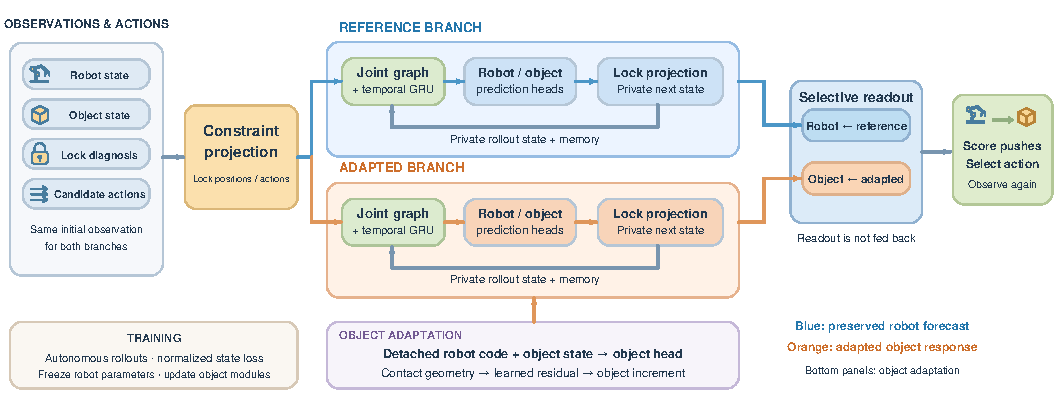
\includegraphics[width=.98\textwidth]{figures/lockpusher_revision/state_isolation.pdf}
\caption{状态隔离预测。两分支在相同观测、动作和锁定诊断下分别维护独立滚动状态。返回的机器人坐标来自参考分支，物体坐标来自干预分支。部署配置的机器人分支不接收物体状态输入。}\label{fig:isolation}
\end{figure*}
\subsection{匹配适配}
大规模适配实验的各变体从同一预训练载体开始。我们冻结机器人参数并更新物体预测头。LockPusher额外更新几何物体残差；无残差变体不含该修正；全局变体学习全部状态坐标的修正。各方法共享数据和优化预算。

底层适配模型直接训练，其预测$\tilde s_t$通过自主预测窗口上的归一化状态平方误差优化；状态隔离用于返回候选预测：
\begin{equation}
\mathcal L=\frac{1}{14H}\sum_{t=1}^{H}\|D^{-1}(\tilde s_t-s_t)\|_2^2.
\end{equation}
对角尺度矩阵$D$对关节位置、关节速度、物体位置、物体速度分别使用0.1 rad、1 rad/s、0.03 m、0.1 m/s。物体适配变体中，机器人误差不更新被冻结的机器人参数；全局残差也接受机器人坐标监督。训练共十轮，前五轮预测长度为10，后五轮为25。每条轨迹每轮提供一个随机位置的连续窗口。验证以25步物体位置MSE最小为选模标准，包含初始检查点。新适配权重与历史部署权重分别评估。

\subsection{候选选择与执行}
对每个候选，LockPusher展开并计算$\hat c_k=\|\hat p_H^{(k)}-g\|_2$，选择$k^*=\arg\min_k\hat c_k$。执行后由新观测重新初始化两分支。受控仿真每轮以50步预测评估128个候选，执行10步，共五轮。真机控制器使用其记录的候选构造方式，朝序列索引24处的参考点运动后再次观测。两者均采用重复观测与预测，但执行协议不同。


\section{实验}

\textbf{仿真有效性。}主实验初态核查发现工具与物体、桌面穿透，以及部分关节越限。下述主实验、校准、数据预算和同权重候选结果保留为存档数值比较，尚不能作为有效物理性能证据。历史预测使用不同重置过程，其物理有效性仍未核实；真机执行另行评价。

\textbf{评价量的定义。}仿真终点误差为$e_{\mathrm{goal}}=\|p_T-g\|_2$，其中$p_T$为实际执行后的物体位置，$g$为任务目标；它不是模型预测误差。目标距初始物体位置40--65或65--90 mm。均值包含失败任务，成功条件为$e_{\mathrm{goal}}<30$ mm。预测RMSE则比较预测坐标与实测真值。真机采用不同的图像空间标准：各轴误差不超过五像素并连续满足三个不同观测帧，核心目标位移20像素（约35.1 mm）。因此，真机与仿真成功率不能直接比较。

投影标称模型、无对象残差与全局适配三项匹配对照分别检验适配、对象修正与修正范围对应的存档终点差异。历史输出与递推对照则固定权重和输入，检验参考预测的保持。

\subsection{仿真设置}

仿真机械臂推动具有两个平移自由度、朝向固定的方块。实验覆盖五种单关节锁定与四类物理设置：标称、高阻尼、弱电机和混合扰动。高阻尼将关节阻尼设为标称值的两倍，弱电机将驱动增益设为70\%，混合条件同时施加两者。适配、验证、测试分别包含50,000、2,000和6,000条独立重置轨迹，重置种子互不重叠。每条轨迹为50步，步长5 ms。各变体从共享预训练基础出发，按上述匹配适配方案进行六次拟合。

对照包括LockPusher、去除对象残差、全局残差适配和投影标称动力学。闭环评估包含1,200个共享起点—目标问题，每个锁定与距离区间组合120个。每个组合为四类物理设置各分配30个问题，目标方向在前向正负45度内均匀采样。控制器每次重规划评估128条候选命令，预测50步、执行10步，然后重新观测；每段任务固定执行五次重规划，共0.25 s；每次预测0.25 s，仅执行前0.05 s，进入目标区域也不提前终止。每个候选由五段命令组成，各段保持十步；未锁定关节命令独立均匀采样自$[-0.8,0.8]$，锁定关节置零。各方法共享问题和候选采样设置，但从各自实际到达的状态继续规划。终点误差为对象到目标的欧氏距离，小于30 mm计为成功。位置与速度RMSE分别以mm与m/s报告。

\subsection{存档闭环对照}

六次适配拟合中，LockPusher相对去除对象残差将平均终点误差从49.95 mm降至47.02 mm。各拟合的配对改善为1.79--5.25 mm，按问题自助采样的区间均为正；平均成功率从24.88\%升至27.64\%。这些差异存在于存档仿真输出中，尚不能证明物理任务进展得到改善。

初始距目标平均65.07 mm，LockPusher执行后剩余47.02 mm，平均缩短18.05 mm。成功率对应30 mm目标区域，尚不表明精确定位。物体平均净位移为60.96 mm，因此不能仅用执行时间短解释剩余距离。ActivePusher的Fig. 7报告沿路径的平均SE(2)跟踪误差，其区域任务目标为100$\times$100 mm\cite{zhong2026activepusher}；这里的终点目标距离不能与该混合位姿指标直接比较。

相对投影后的名义动力学，LockPusher使平均终点误差降低7.93毫米，平均成功率提高8.00个百分点；六次拟合的终点配对改善区间均为正。

全局残差适配的平均终点误差为45.58 mm，成功率30.71\%。它在六次拟合中的五次获得更低终点误差，其中四次配对区间不跨零。因此，限制适配状态可以保留指定机器人预测，但不意味着在所有模型类别中获得最低终点误差。开环位置RMSE同样未在对象适配后普遍改善。

固定检查点预测实验在补充分析中报告，位置与速度在全部物理条件下分别评估。真机实验使用历史部署权重，详见真机实验章节。
\input{sections/planning-table-zh.tex}
\begin{figure*}[t]\centering
\includegraphics[width=.98\textwidth]{figures/meeting_revision/planning_three_comparisons.pdf}
\caption{LockPusher的三组配对终点对照：(a)相对投影标称模型的适配对照；(b)相对无对象残差模型的对照；(c)与全局适配的比较。正值表示LockPusher更好。每点对应一次拟合在1,200个共享问题上的平均值，误差线为2,000次配对问题bootstrap的95\%区间。三个面板使用相同坐标尺度。}\label{fig:paired-plan}\end{figure*}

\subsection{验证集选择的残差缩放}
这项残差缩放研究中，候选随机采样随拟合种子变化，同一拟合内各方法共享随机抽样。分层bootstrap在十个锁定—距离组合内重采样问题，并让同一问题索引携带全部方法和拟合结果；区间以这些拟合及其候选采样为条件。

独立的训练后研究按既有验证集H50位置MSE，从$\{0,0.5,1,1.5\}$中选择各拟合的对象残差强度。在2,000条新的共享轨迹上，平均逐坐标位置RMSE由21.845降至20.750毫米。在另1,200个共享闭环问题上，平均终点误差由46.75降至46.22毫米，成功率由28.21\%升至28.97\%。终点配对改善为0.532毫米；以六个拟合为条件，问题bootstrap的95\%区间为[0.357, 0.712]毫米。三个改变强度的拟合具有正区间，一个跨零，两个保留原强度。在这些新问题上，相对无对象残差模型，校准后的LockPusher使终点误差降低3.398毫米（条件95\%区间[3.085, 3.710]毫米），六次拟合的区间均为正，平均成功率提高3.90个百分点。第二组问题共享初始化缺陷，不能独立验证物理收益。全局适配在相同问题上达到45.34毫米和30.60\%成功率。校准小幅降低终点误差，全局适配的平均终点误差仍更低。校准权重未部署至真机。

\begin{table}[t]\centering\small
\caption{校准相对原模型的逐拟合闭环变化。正值表示改善；区间为条件95\%配对问题bootstrap区间。}\label{tab:calibration-fits}
\begin{tabular}{rrcr}\toprule
拟合 & 缩放 & 误差降低（mm） & 成功增量（pp）\\\midrule
7 & 1 & 0.00 [0.00, 0.00] & 0.00\\
17 & 1.5 & 1.40 [0.91, 1.91] & 1.50\\
27 & 1.5 & 0.69 [0.23, 1.16] & 1.50\\
37 & 1.5 & 0.98 [0.44, 1.56] & 2.50\\
47 & 1 & 0.00 [0.00, 0.00] & 0.00\\
57 & 1.5 & 0.11 [-0.42, 0.64] & -0.92\\
\bottomrule\end{tabular}\end{table}

\textbf{全状态与选择性输出。}另一组历史评测使用检查点27、37、47，覆盖高阻尼、组合与未见组合条件，各条件十条轨迹，预测长度为10、25、50。所得27个组合不代表独立训练重复。表~\ref{tab:historical-publication}汇总全部27个组合。两种输出的对象状态RMSE相同，相对载体平均降低16.74\%。全状态输出在三个组合中增加自由状态RMSE，并在两个组合中增加推杆RMSE；选择性输出始终保留载体的这两项误差。其余24个组合中，全状态输出改善了自由状态RMSE，因此保持并不意味着精度占优。对象与自由状态指标均混合位置和速度，不能解释为毫米位置误差。全状态输出返回干预分支的机器人与物体坐标，选择性输出返回载体机器人坐标与相同的干预物体坐标。两分支均保留各自的滚动状态；下述递推消融则改变下一步的状态输入。这些历史预测测试不能证明物理控制收益。

\begin{table}[t]\centering\small
\caption{历史输出对照的全部27个组合。误差降幅与增幅均相对载体；对象降幅为三个检查点均值的平均。匹配数指所有存档窗口的自由状态与FK推杆平方误差均与载体相同的组合数。}
\label{tab:historical-publication}
\setlength{\tabcolsep}{3pt}
\begin{tabular}{lrrrr}\toprule
方法 & \shortstack{对象RMSE\\降幅(\%)} & \shortstack{自由状态\\退化数} & \shortstack{最大自由\\增幅(\%)} & \shortstack{自由/FK\\匹配数}\\\midrule
载体 & 0.00 & 0/27 & 0.00 & 27/27\\
全状态 & 16.74 & 3/27 & 6.20 & 0/27\\
选择性 & 16.74 & 0/27 & 0.00 & 27/27\\
\bottomrule\end{tabular}\end{table}

\textbf{共享状态与独立递推。}回顾性对照使用84条先前已评估轨迹，七个物理条件各12条，并在不同递推方式间固定历史权重、上下文、观测和动作。共享状态版本保留两套递归记忆，但将拼接后的机器人与物体状态共同输入下一步转移。三个拟合与三个预测时域复用这组轨迹。全部63个拟合、条件与时域组合中，共享状态与独立递推的物体位置和速度RMSE相同。独立递推在全部组合中精确保留单独运行的载体机器人预测，共享状态版本则在全部63个组合中改变该预测。相对共享递推，独立递推的机器人诊断RMSE在30个组合中改善、33个组合中变差。因此，隔离控制的是参考预测保持，并不意味着参考本身更准确；存档闭环残差对照另行报告对象适配后的终点差异。

\section{真机闭环推动}
我们使用五自由度机械臂，在完整臂和单关节锁定条件下评估短距离推动。任务要求沿任务轴移动20像素，按记录标定约为35.1毫米。六种条件各有三次有效试验，全部18次核心试验均达到下文定义的成功判据，结果见表~\ref{tab:real-push}。

控制器使用视觉物体观测和关节反馈，以50步时域评估至少10,000条候选关节参考序列，按每秒5度的速度限制朝所选参考点运动，随后重新观测并规划。图~\ref{fig:hardware-sequence}展示记录的执行过程，图~\ref{fig:real-scene}展示实验平台。

起点门限为每个图像轴两像素。成功要求物体到目标的误差在每个轴上均不超过五像素，并保持三个不同的连续观测帧。存档终点统计则使用最后十个检测观测的逐坐标中位数。成功由连续帧判定，不使用该中位数。每种核心条件的三次重复复用一份准备阶段候选档案，在线根据当前关节状态和剩余误差变换；不同条件使用不同档案。

\begin{table}[t]\centering
\caption{记录的闭环推动结果。双锁定目标更短且控制配置曾改变，属于诊断案例，并非同一固定控制器的重复试验。}
\label{tab:real-push}
\begin{tabular}{lrrrr}\toprule
条件 & 目标(px) & 成功 & 有效次数 & 周期\\\midrule
完整臂 &20&3&3&4\\
J1锁定 &20&3&3&4--5\\
J2锁定 &20&3&3&17\\
J3锁定 &20&3&3&16--18\\
J4锁定 &20&3&3&7\\
J5锁定 &20&3&3&6--7\\\midrule
J1+J2 &15&1&1&14\\
J2+J3 &15&1&1&34\\
J3+J4 &15&1&3&5--31\\\bottomrule
\end{tabular}
\end{table}

真机候选指定关节参考$q^{\mathrm{ref}}_t$。预测时，PD规则根据返回的机器人状态生成模型动作：$a_t=\Pi_d(\operatorname{clip}(5(q^{\mathrm{ref}}_t-\hat q_t)-0.5\hat{\dot q}_t,-1,1))$。因此，真机候选评分包含预测展开内部的状态反馈。在初始状态与循环记忆匹配、分支确定的条件下，对于相同参考序列，该机器人状态反馈规则仍保留参考预测，因为每步相同的参考机器人状态产生相同动作。部署模型的机器人分支不依赖物体状态，故共享状态与独立递推在相同参考下产生一致的机器人预测。

候选参考是按剩余任务轴误差缩放的关节偏移，锁定关节参考固定在诊断角度。每次观测由标定图像测量初始化物体位置，并将物体速度置零。控制器朝索引24处的参考点运动后重新观测，不会依次执行此前参考点。历史严格仿真采用开环候选执行，当前大规模仿真每执行十步后重规划，二者均不同于该真机命令。

全部23次正式真机试验记录相同模型配置，并使用\texttt{icra\_confirmation\_d3\_query\_selective\_w10}中的seed-27选择性检查点。其张量与历史严格仿真使用的seed-27残差训练检查点相同。这组存档部署权重与新适配拟合分别报告。

另有五次有效双锁定试验，要求较短的15像素位移，约26.3毫米。J1+J2与J2+J3各成功一次，J3+J4有两次失败与一次成功。这些诊断案例的候选和控制设置发生过变化，因此逐项报告，不合并为固定控制器重复。失败、无效和中止尝试均保留在清单中。真机未采集匹配基线；真机试验展示了记录协议下的执行，但不能据此确认存档仿真对照的物理有效性。

\begin{figure*}[t]\centering

\includegraphics[width=.98\textwidth]{figures/lockpusher_revision/hardware_sequence.pdf}
\caption{J3单关节锁定的真机执行。俯视帧分别对应初始观测、达到任务轴目标位移的一半、首次连续三帧达标；各帧选自监测事件前最近一次相机采集。放大图中的蓝线与橙框分别标记记录的起始坐标和目标容差，腕部视图展示初始构型。}\label{fig:hardware-sequence}
\end{figure*}
\begin{figure*}[t]\centering

\includegraphics[width=.98\textwidth]{figures/lockpusher_revision/environment_plate.pdf}
\caption{物理平台与CAD示意。(a)按归档准备构型渲染的完整机械臂。(b,c)归档J3试次在不同时刻的腕部与俯视图。定量仿真使用几何结构不同的独立机械模型；CAD图用于展示硬件构型。}\label{fig:real-scene}
\end{figure*}

存档还包含同权重候选对照：在120个新D3问题上，每问题128个候选并开环执行50步，已部署seed-27检查点相对投影名义模型使终点误差降低8.72毫米（配对问题95\%区间[6.48,11.04]毫米）。种子7、17、27相对匹配载体分别降低2.42、1.65、0.27毫米，仅种子7的区间完全为正。该对照共享可疑初始化，不能据此确认部署权重的物理收益。

\section{局限与结论}
LockPusher研究已诊断关节锁定下对象适配的作用范围。独立滚动状态保留指定机器人预测，同时保留干预分支的物体预测。历史配对对照展示了预测层面的作用：对象状态误差降幅可以保留，而不继承已观察到的、相对载体的机器人误差增加。真机试验展示了由结构直接满足保持性质的模型配置下的视觉重规划，并未分离独立滚动的收益。大规模仿真对照存在初始化缺陷，物理控制增益仍未得到验证。

当前证据覆盖固定朝向的仿真方块和单机械臂短距离真机推动。正确诊断是输入假设，保持载体并不证明其准确。将该形式扩展至可旋转物体及需要适配机器人接触动力学的任务，是后续研究方向。

\section*{致谢}
OpenAI Codex用于摘要、引言、相关工作、方法、实验、结论及附录的起草与修订，中文翻译，图表代码编写，以及所提供实验记录的整理。

\renewcommand{\refname}{参考文献}


\appendix
\section{固定检查点预测分析}
这些历史检查点不同于主闭环实验的新适配模型。例如，种子47在弱电机、50步条件下的位置RMSE由8.63升至28.20 mm，而速度RMSE由0.152降至0.073 m/s；分量间的取舍不能由混合单位的综合指标概括。


固定检查点实验在D3锁定和固定侧接触邻域策略下生成8,400条独立轨迹，七个物理条件各1,200条，三个已有检查点分别评估10、25、50步。全部63个组合中，选择性包装器相对载体的机器人坐标改动和最大锁定违反均为零。

位置与速度分开后的结果表明，收益取决于检查点、物理条件和预测长度，一个分量的改善可能伴随另一个分量恶化。历史组合指标在高阻尼、组合与未见组合的27个预指定组合中均下降，平均16.27\%，但该指标混合了位置与速度单位。正文图分别展示具有物理单位的分量结果。固定检查点与闭环适配拟合分别报告。

\subsection{适配数据预算}
\input{sections/data-budget-table-zh.tex}
我们在固定优化更新步数下改变适配训练轨迹数。按锁定关节与物理条件均衡抽取的嵌套训练子集分别包含1,000、5,000和50,000条轨迹，各预算另使用400条验证轨迹。各方法进行三次拟合，复用seed-27来源模型已训练的机器人与物体动力学参数，并重新初始化新增残差头。每次以512的批量大小更新980步，前后各490步分别采用10步与25步预测。每次拟合均按验证集上的H25物体位置MSE选择最优检查点，再在1,200个新的共享问题上按相同闭环协议评估。上述计数不含来源模型此前的全部训练与开发数据。

表~\ref{tab:data-budget}报告全部拟合。对两个较低预算等权平均，LockPusher相对去除物体残差降低终点误差3.23毫米。六个拟合与预算组合均改善，配对95\%问题bootstrap区间均不跨零（在40个锁定关节、距离与物理条件分层内重采样2,000次，以各拟合为条件）。在50,000条轨迹下，两次拟合改善，一次退化。LockPusher的平均终点误差未随训练预算单调下降，全局适配在各预算下的平均终点误差均更低。这些存档拟合在两个较低预算下得到更低终点误差，但未呈现单调的规模趋势；物理收益仍待验证。

\begin{figure*}[t]\centering
\includegraphics[width=.98\textwidth]{figures/meeting_revision/historical_absolute.pdf}
\caption{历史模型的全部63个组合。数值为载体RMSE减去适配RMSE，正值表示改善，负值表示退化；位置以mm、速度以mm/s分别报告，各面板使用独立色标。27、37、47为历史种子标识，不是训练轮次。星号表示历史预指定条件。}\label{fig:prediction-conditions}\end{figure*}

\input{sections/appendix-method-zh.tex}
\input{sections/historical-evidence-zh.tex}


\bibliographystyle{IEEEtran}
{\small\linespread{1}\selectfont\bibliography{references}}
\end{document}
